\documentclass[../main.tex]{subfiles}

\begin{document}

  \subsection{Designklassediagram} \label{designmodel-detaljeret}
  
  \subsubsection{GUI, Aquiantance og utility}
  \begin{figure}[H]
    \centering
    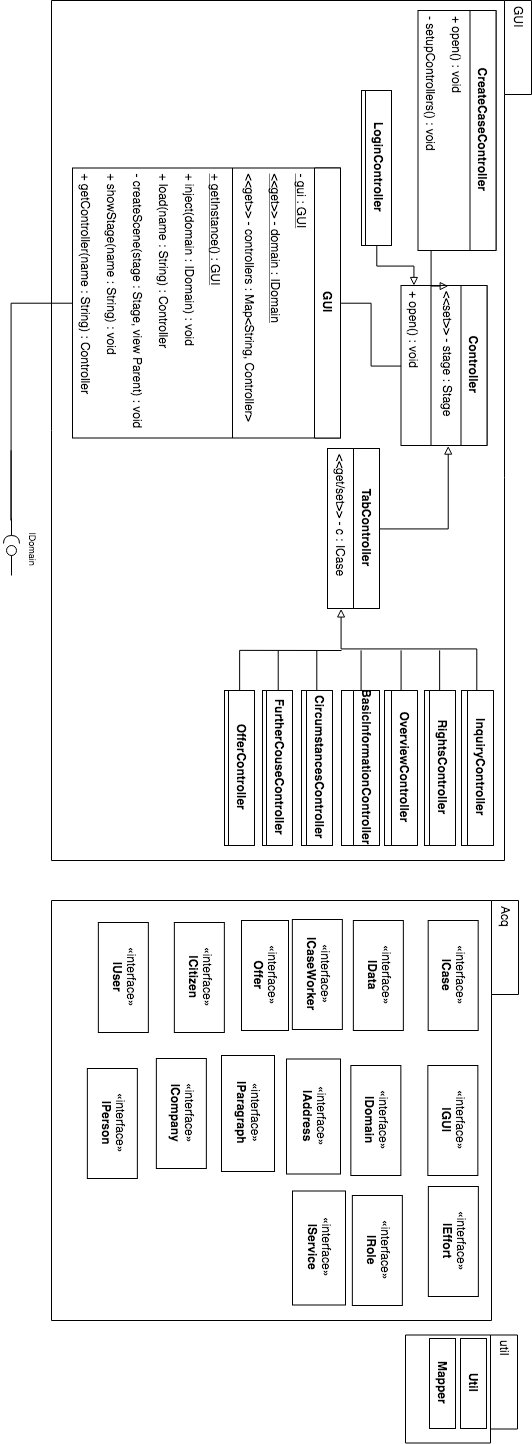
\includegraphics[scale=.34]{figurer/design-gui.png}
    \label{fig:design_gui}
  \end{figure}
  
  \subsubsection{Domain}
  \begin{figure}[H]
    \centering
    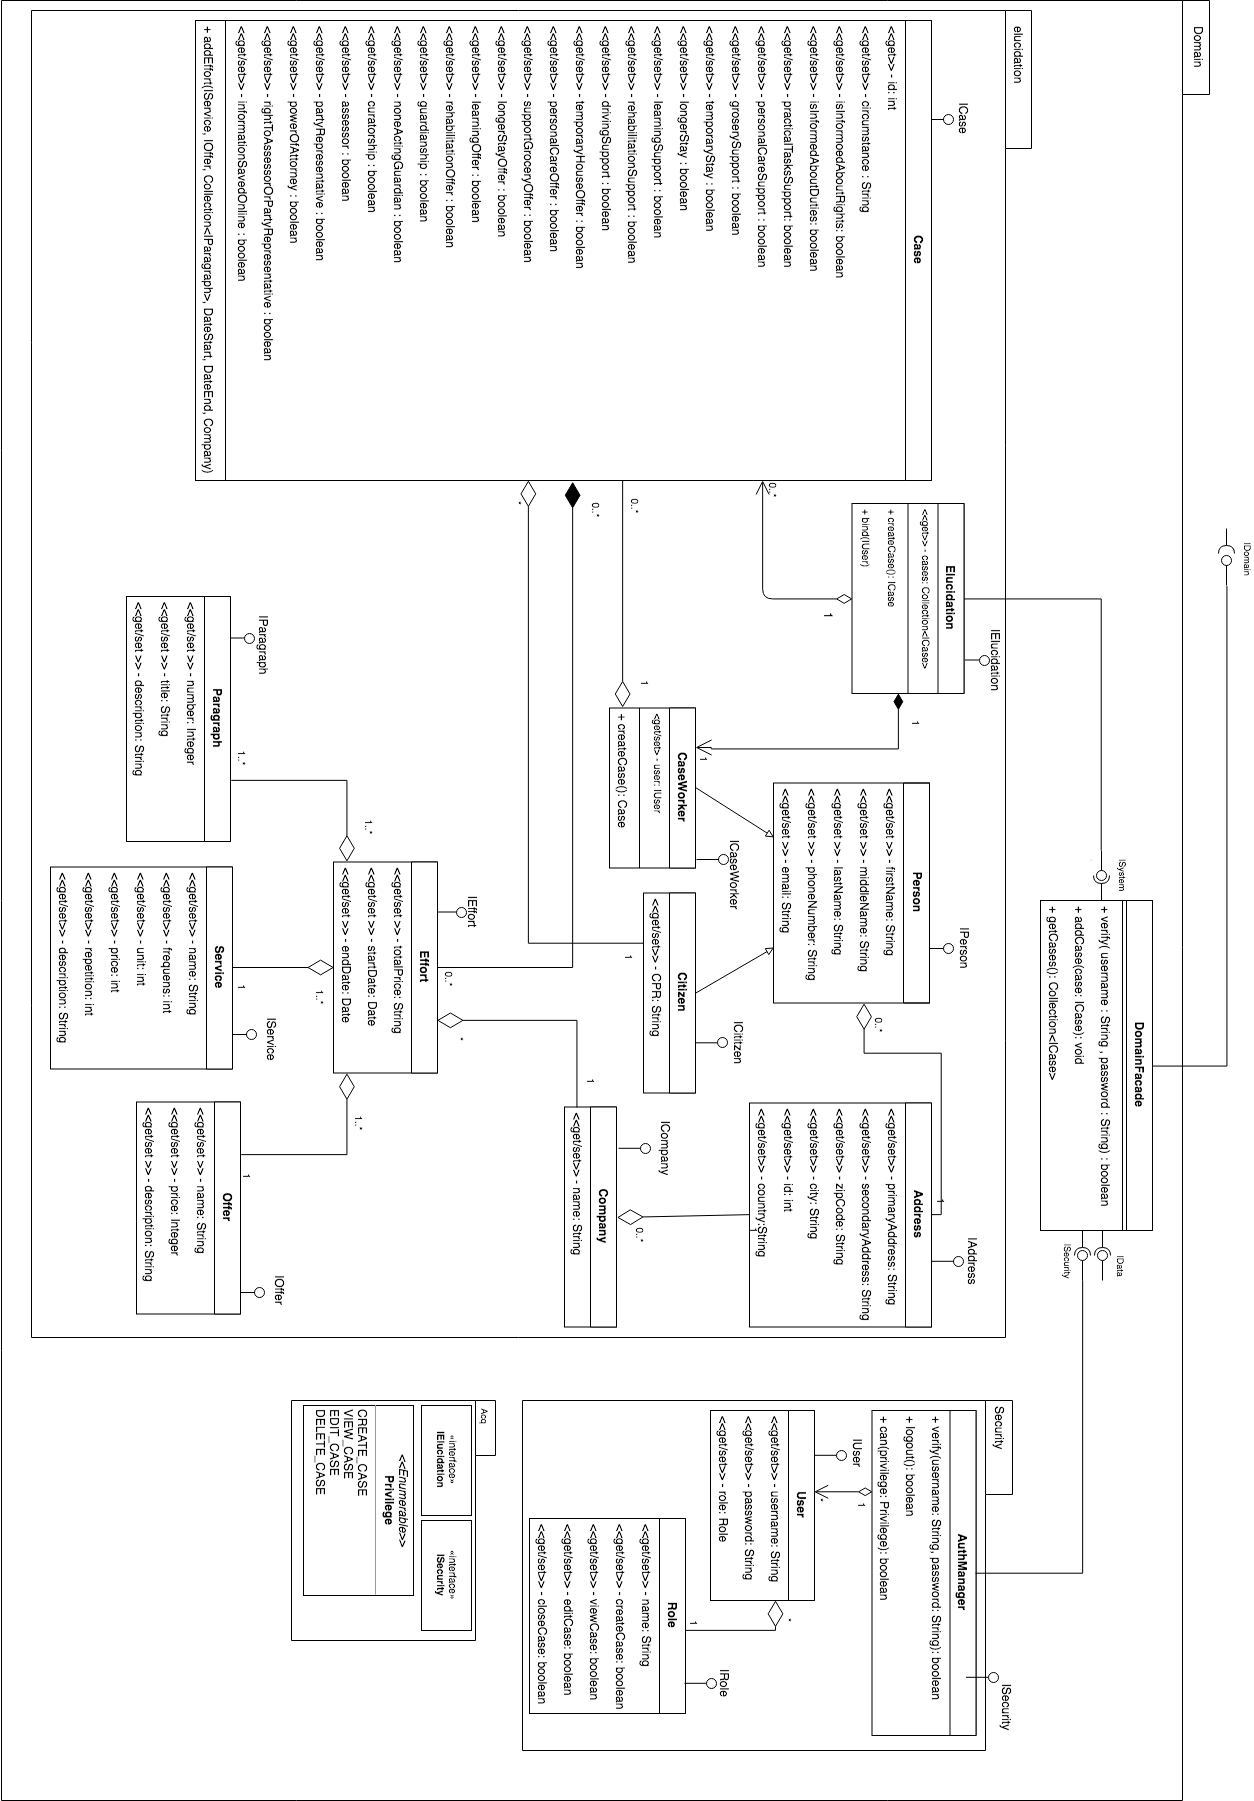
\includegraphics[scale=.30]{figurer/design-domain.png}
    \label{fig:design_domain}
  \end{figure}
  
  \subsubsection{Data}
  \begin{figure}[H]
    \centering
    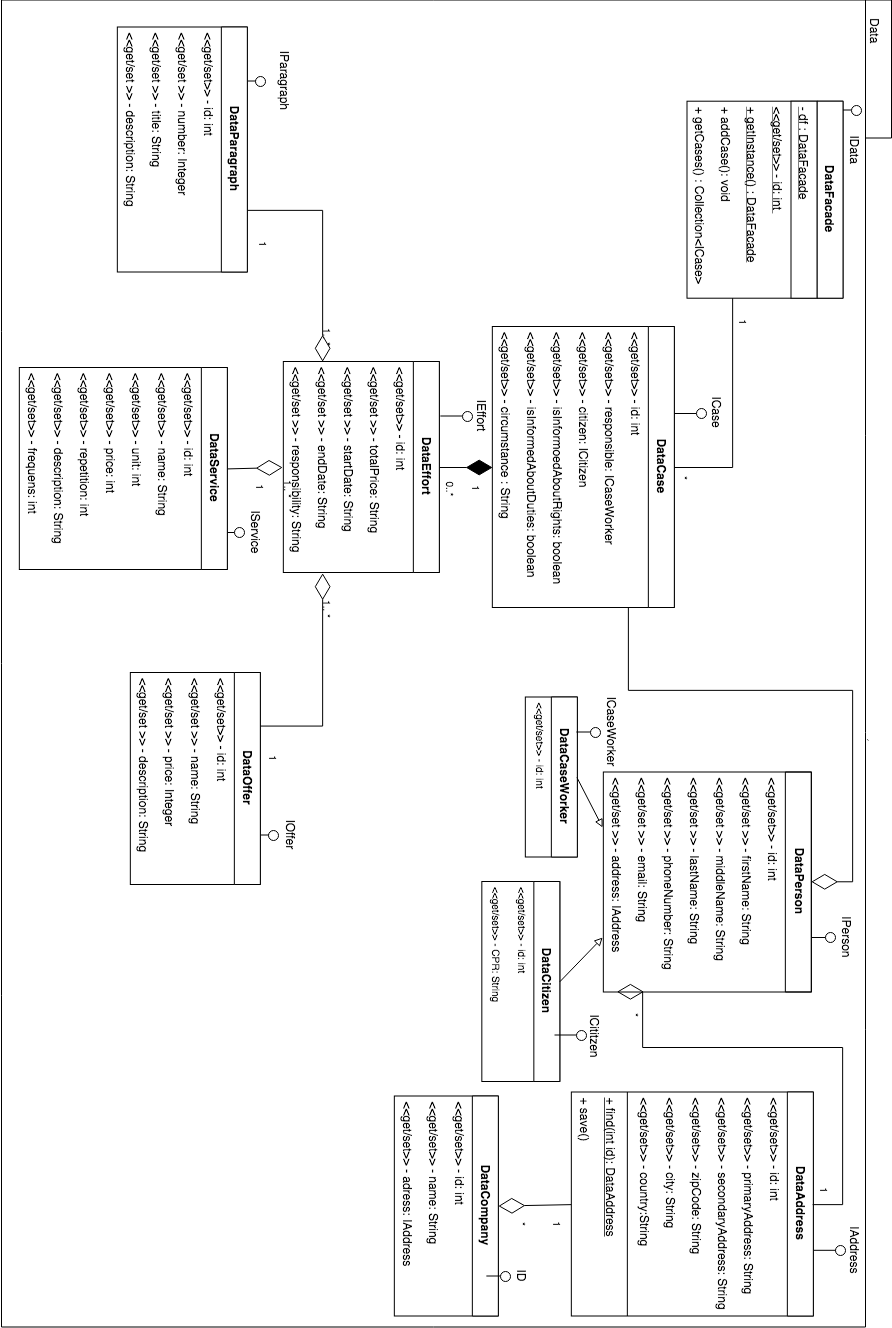
\includegraphics[scale=.4]{figurer/design-data.png}
    \label{fig:design_data}
  \end{figure}
  
  
 \end{document}